\chapter{Appendix C}
\setcounter{figure}{0}
\renewcommand{\thefigure}{C.\arabic{figure}}
\renewcommand{\thesection}{C.\arabic{section}}
\phantomsection
\section{Analysis of Instantaneous Dipole Moment for Ions}
Instantaneous dipole moments for the ions were computed from the simulation trajectory using in-house codes. We calculated the vibration of the Drude particles associated with each ion over the entire simulation trajectory, and the dipole moment for each ion-Drude particle pair was computed as the vector sum of the charge of the particles (ion and the Drude particle) times the distance towards the particle from the combined center of mass of the ion - Drude particle system. The dipole moments are computed in local coordinate frames, such that the center of mass of the ion - Drude particle system is placed at origin. The probability distribution of the instantaneous dipole moments for all the ions is presented in Figure C1.

We analyse the instantaneous dipole moments for the ions as a function of the distance from the graphene surface. We note that for all ions, the probability distributions of instantaneous dipole moments are found to be invariant with the distance from the graphene surface [Figure C1]. We also observe that the distribution of the instantaneous dipole moments are linked to the charge to surface ratio for the ions. For the monovalent ions the spread increases as we move down the period from Li\textsuperscript{+} to Cs\textsuperscript{+}. A higher charge to surface ratio, as observed in the case of Li\textsuperscript{+}, makes it difficult to perturb the charge distribution around the ion resulting in a spread of only 0.03 D. While a lower charge to surface ratio, like in Cs\textsuperscript{+} results in easier perturbation of the charge cloud around the ion resulting in a spread of 0.8 D. Similarly, for divalent cations, we observe that Mg\textsuperscript{2+} has a very narrow distribution for its instantaneous dipole moments, with the distributions bounded between 0 and 0.04 D. While for the larger Ca\textsuperscript{2+} ion, we note that the instantaneous dipole moments have a broad distribution of values ranging between 0 and 0.6 D. For the common counter anion Cl\textsuperscript{-}, we observe that the instantaneous dipole moments are observed in the range of 3.29 to 3.32 D. The large spread in the dipole moments are indicative of a strong response from the Drude particles towards the immediate local environment. In our case this local environment is observed to be the 1\textsuperscript{st} solvation shell. The lack of clear signatures of graphene interactions on the dipole response of ions is due to the fact that the interactions of ions with the graphene surface is mediated by the water molecules.
\begin{figure}
    \centering
    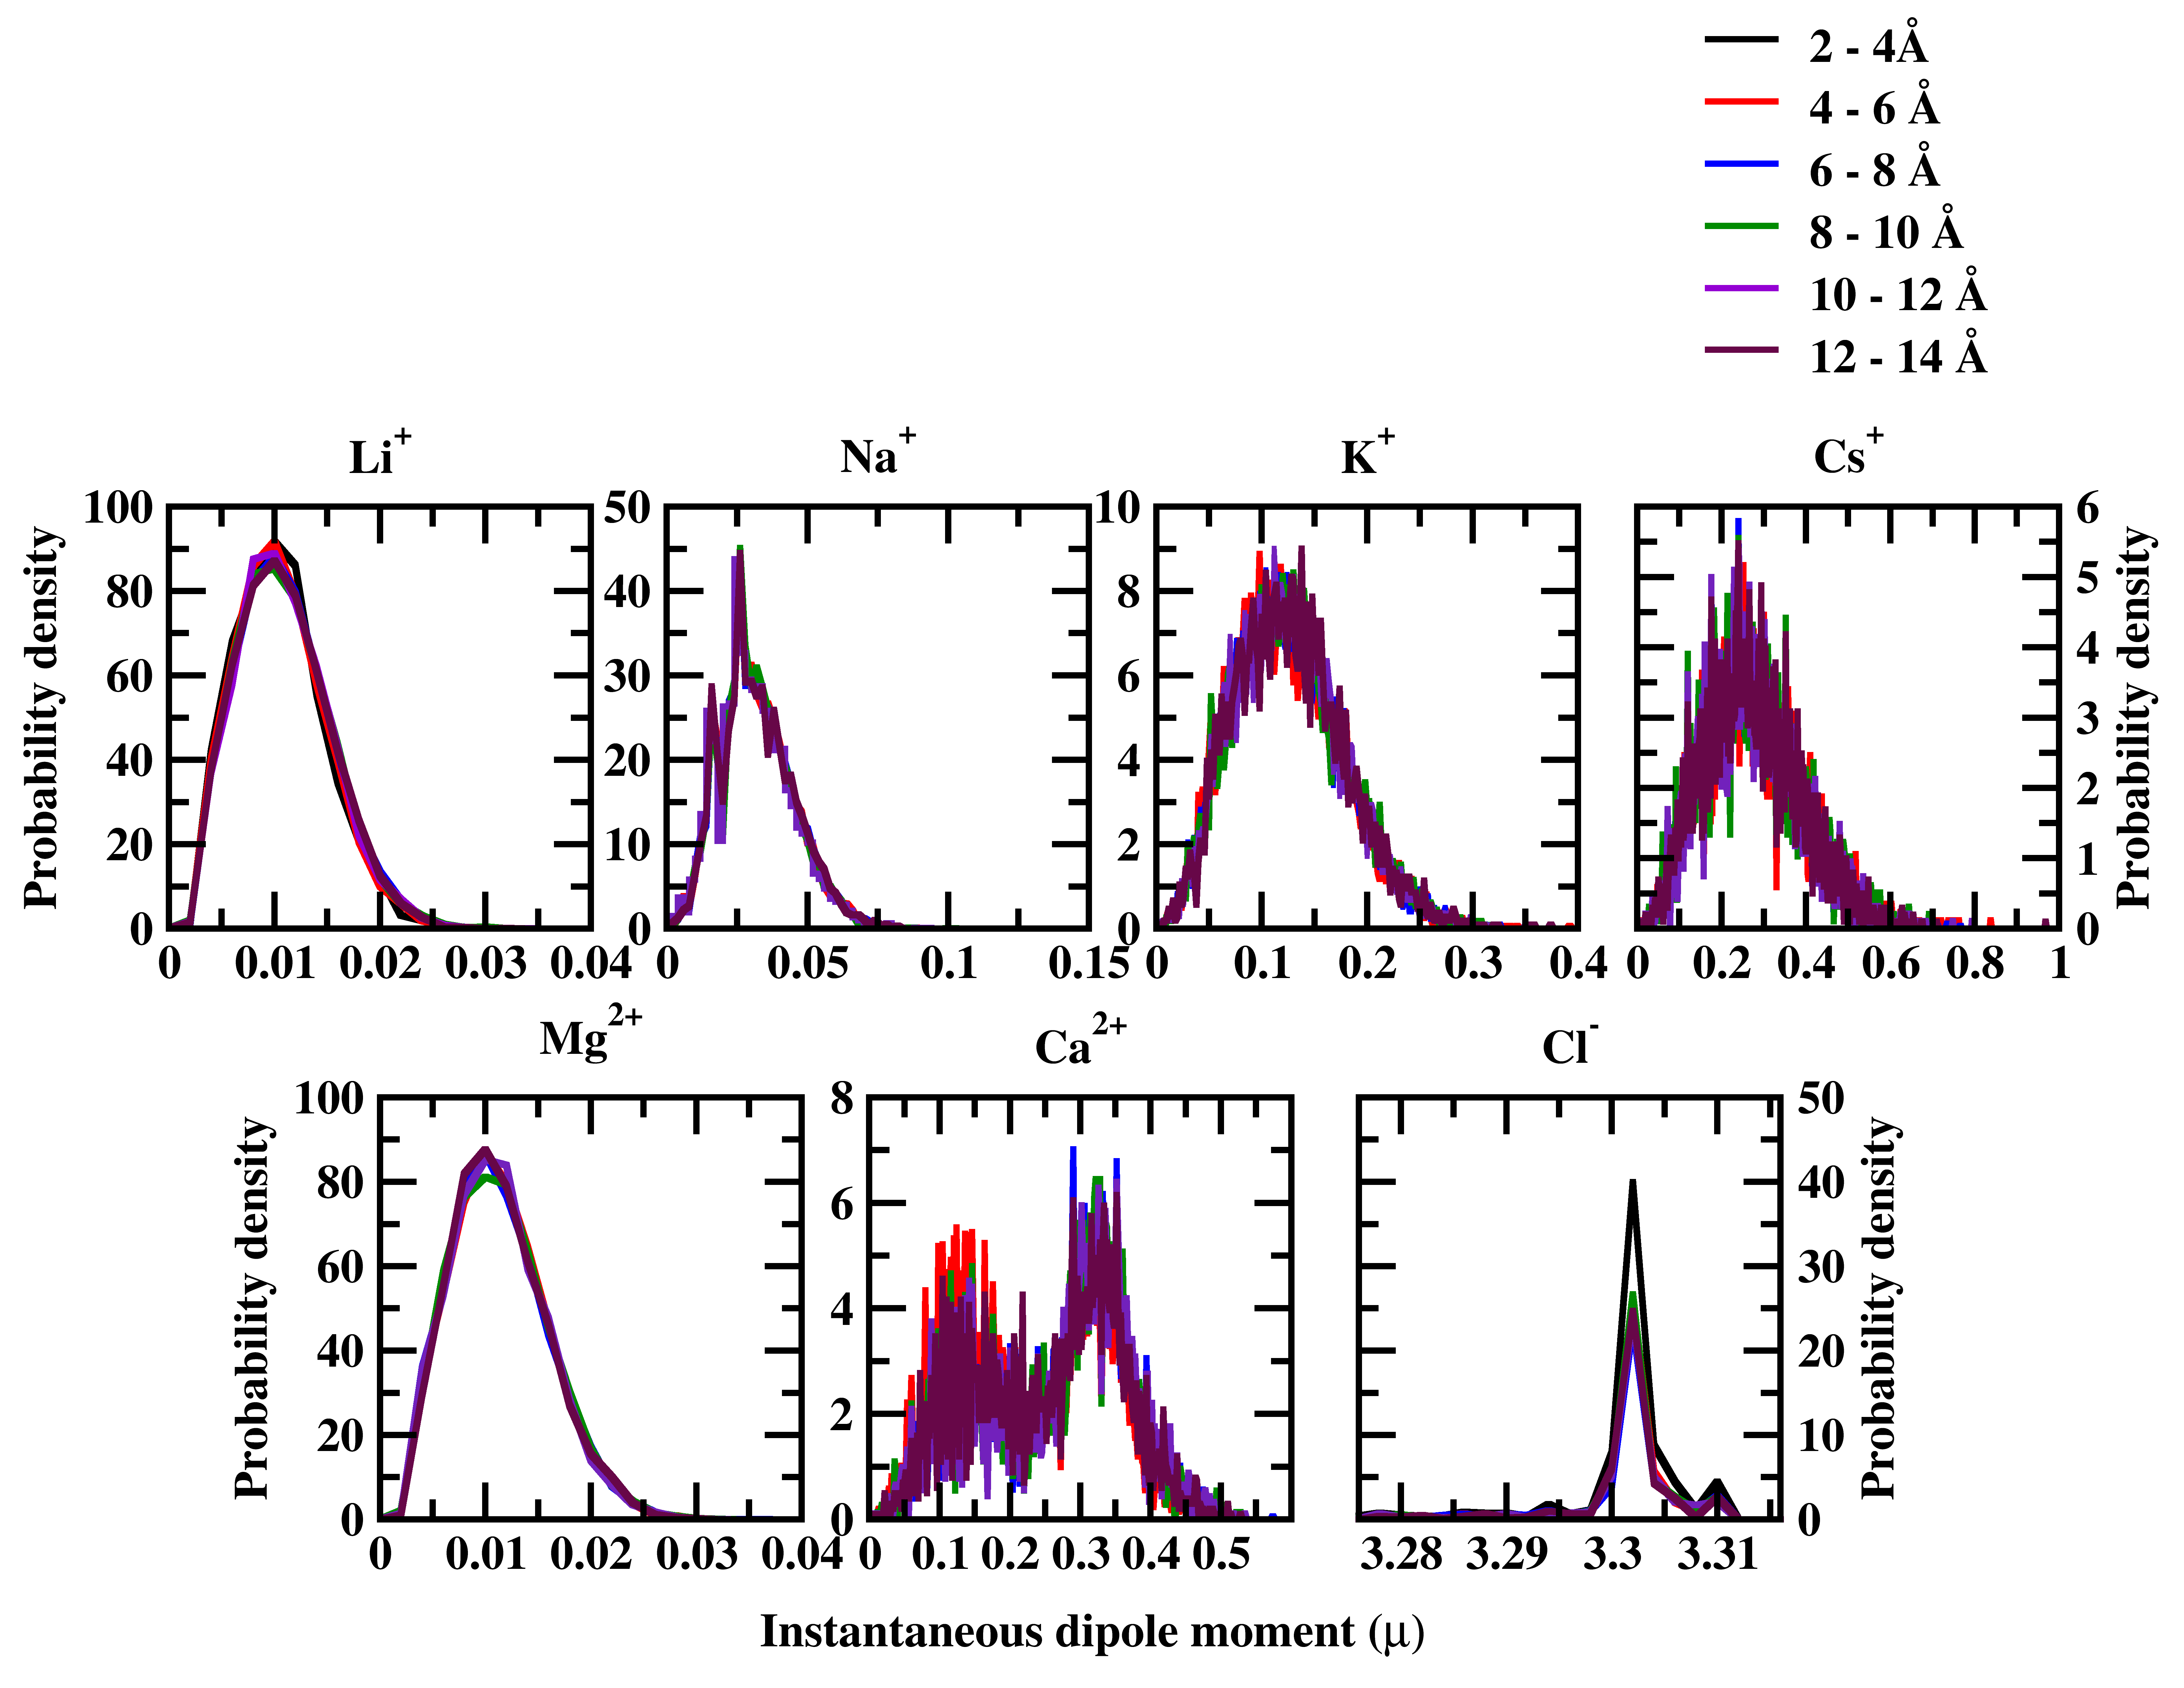
\includegraphics[width=\textwidth]{Appendix/Figures/C1_port.png}
    \caption[Probability distribution for instantaneous dipole moments ($\mu$) for ions considered in this study as a function of the distance from graphene surface, obtained from Drude Polarizable FF simulations]{Probability distribution for instantaneous dipole moments ($\mu$) for ions considered in this study as a function of the distance from graphene surface, obtained from Drude Polarizable FF simulations. All dipole moments are presented in units of Debye.}
\end{figure}

\section{Analysis of Instantaneous Dipole Moment for Graphene Surface}
Average dipole moments for the patches of graphene surface interacting with the ions were computed using in-house codes. Similar to the calculation of the dipole moments associated with the ions, we first iterated over all the ions present in the system, and for each ion, a cylindrical selection of carbon atoms was made, with the radius of the cylinder set to 4 $\angstrom$ and the height of the cylinder set to 14 $\angstrom$. This initial selection was then post-processed to remove water molecules and other ions that might be present, to generate the patch of graphene surface directly interacting with the ion. The dipole moment for the graphene patch was then computed as a vector sum of the charge of the particles (carbon atom and the associated Drude particle) times the distance towards the particle from the combined center of mass of the carbon atom - Drude particle system. It is important to note that the vector sum is calculated over all the carbon atoms present in the patch, with the coordinate frame shifted to each carbon atom in sequence.

\begin{figure}
    \centering
    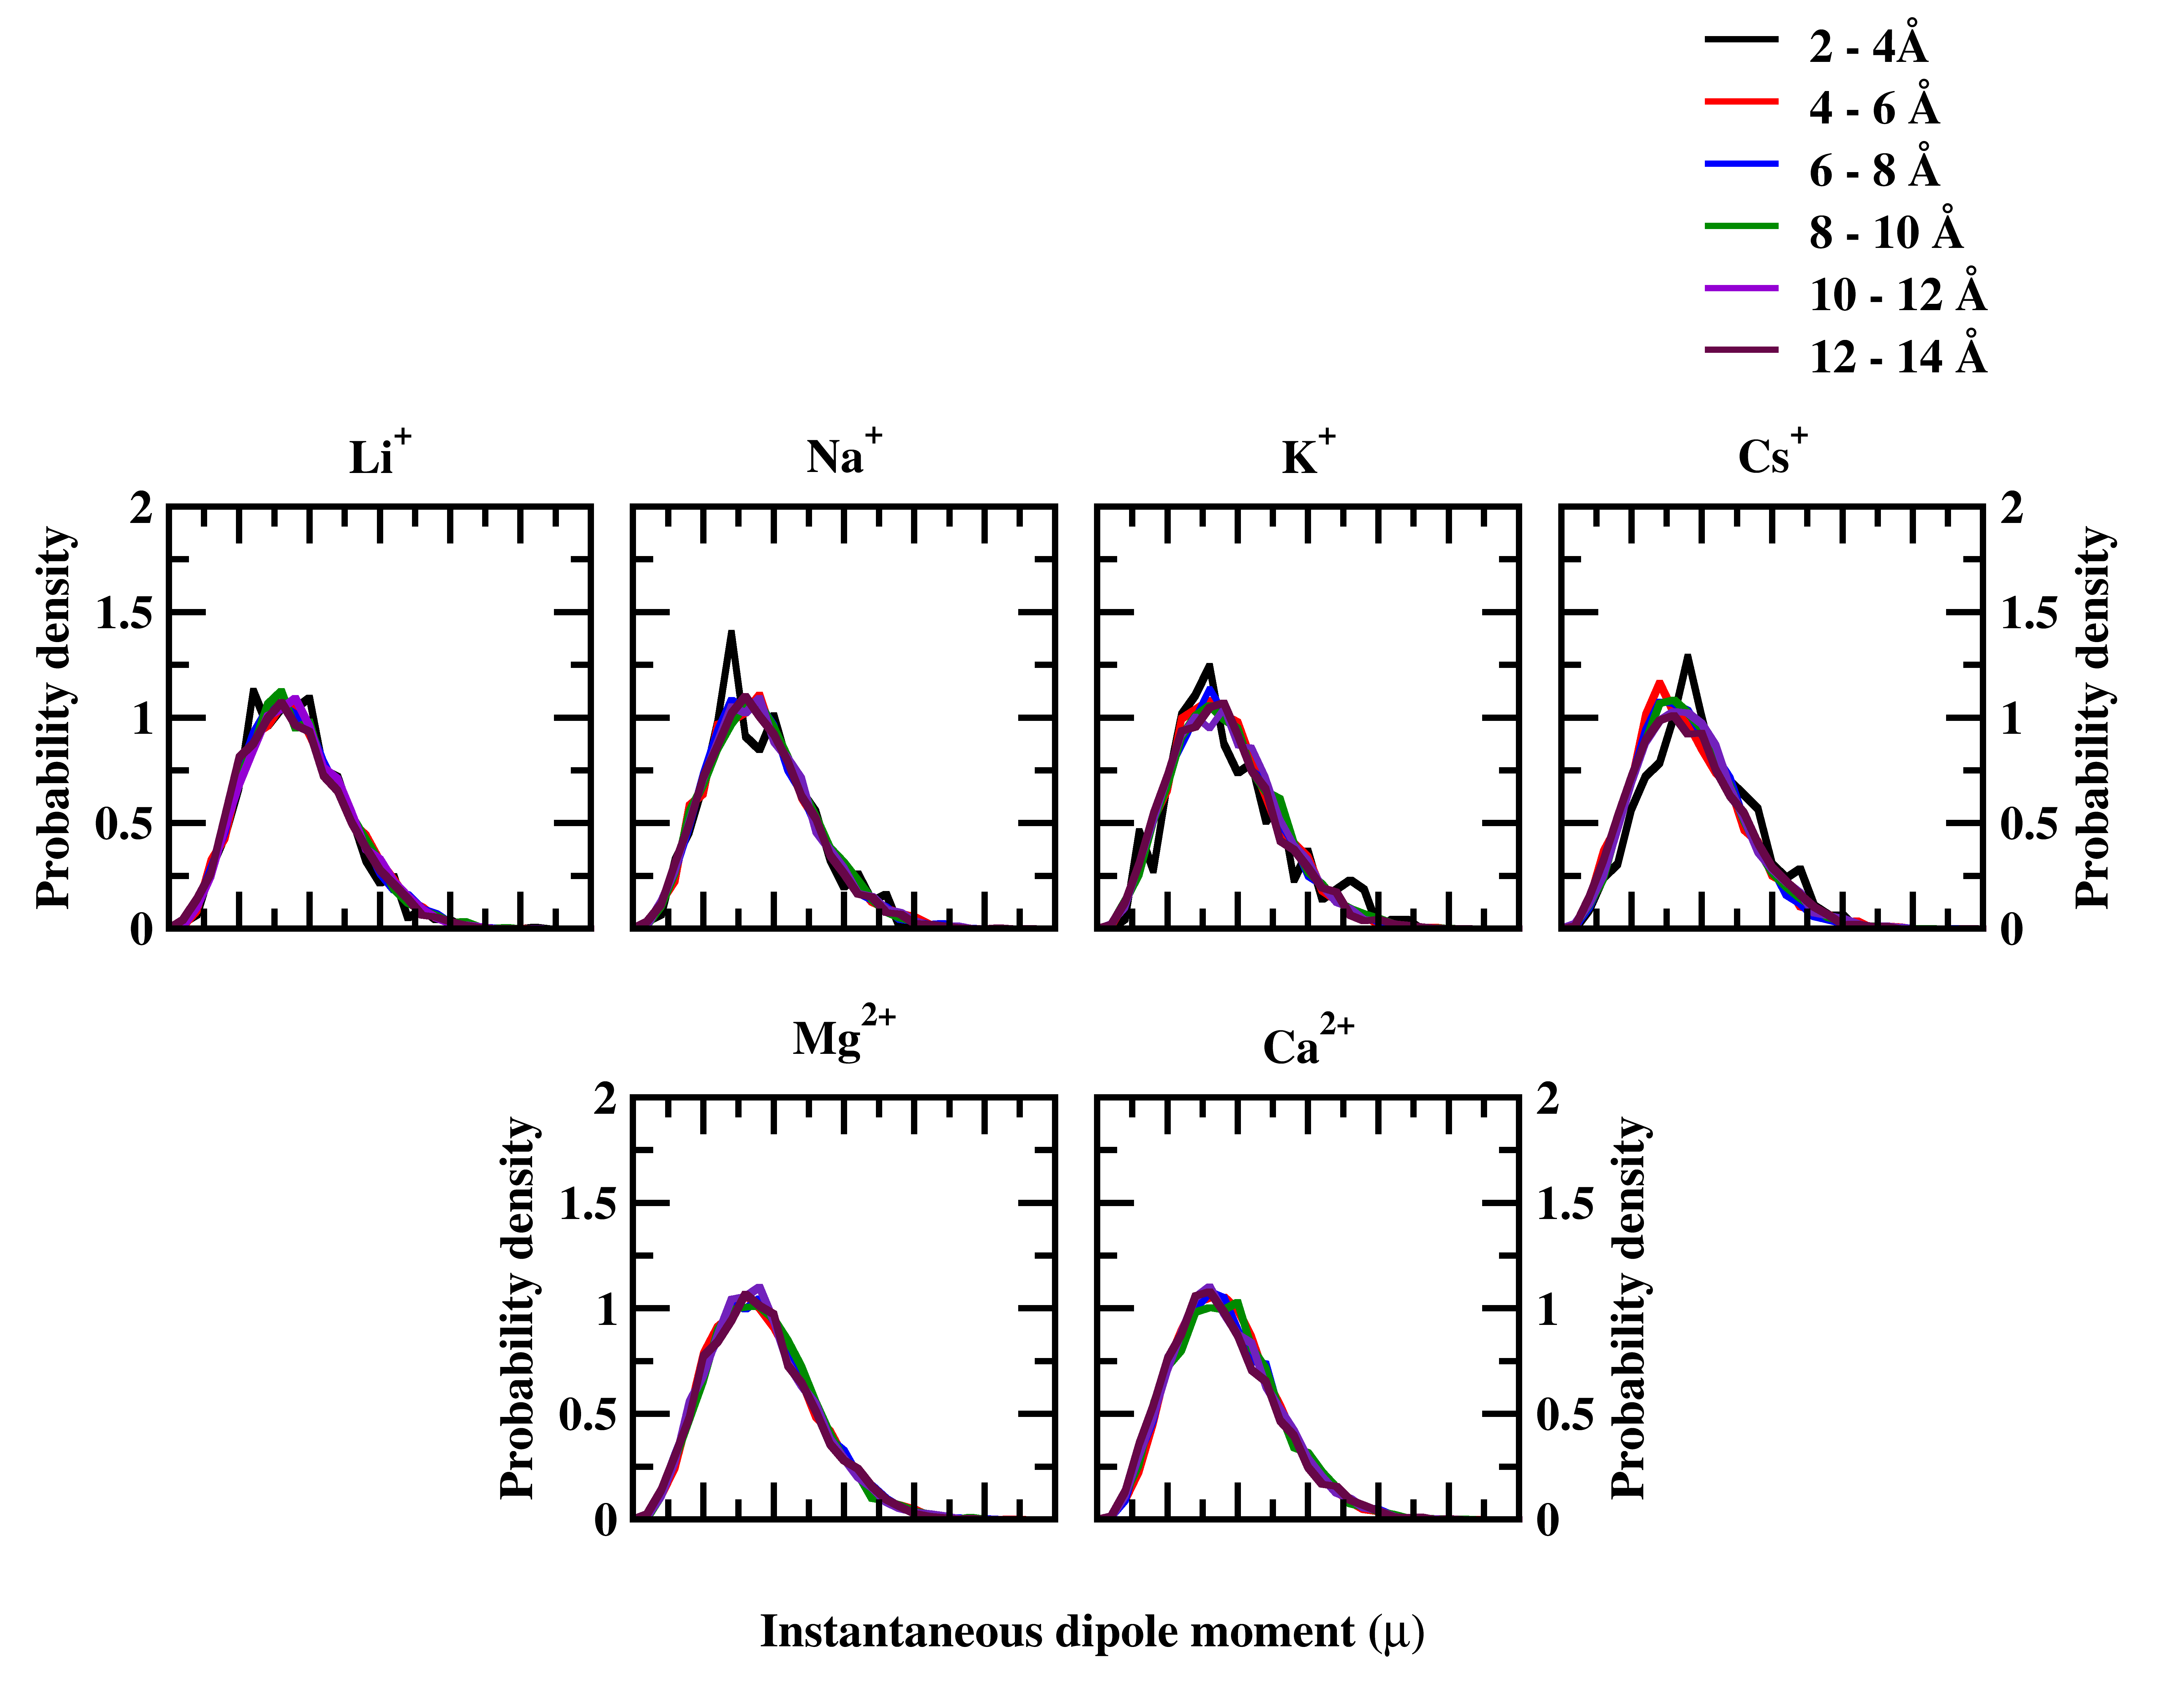
\includegraphics[width=\textwidth]{Appendix/Figures/C2_port.png}
    \caption[Probability distribution of the instantaneous dipole moment ($\mu$) of graphene surface interacting with the ions as a function of distance from the interacting ion obtained from Drude polarizable simulations]{Probability distribution of the instantaneous dipole moment ($\mu$) of graphene surface interacting with the ions as a function of distance from the interacting ion obtained from Drude polarizable simulations. All dipole moments are presented in units of Debye.}
\end{figure}

We present the probability distributions corresponding to the instantaneous dipole moments of the graphene patches as a function of distance from the ions in Figure C2. We observe a significant distribution of the dipole moment, with the value ranging from 0 D to 2.5 D. This indicates a strong coupling with the surrounding environment. However, we note that the average instantaneous dipole moment of the graphene patch is invariant to both the identity of the interacting ion, and the interaction distance. We observe that the variation in the dipole moment is linked to the graphene-solvent interactions. This is also evident for the solvent, wherein the average dipole moment for the water molecules close to the graphene sheet is observed to be close to 2.41D irrespective of the identity of the salt used [Figure 5.7(b)]. Thus, we conclude that the dipole response of the graphene surface is largely dependent on the interacting water molecule.